\documentclass[11pt]{article}

\usepackage[a4paper,margin=2cm]{geometry}
\usepackage{tikz}
\usetikzlibrary{positioning,fit,arrows.meta,calc}

\pagestyle{empty}

\begin{document}

\begin{center}
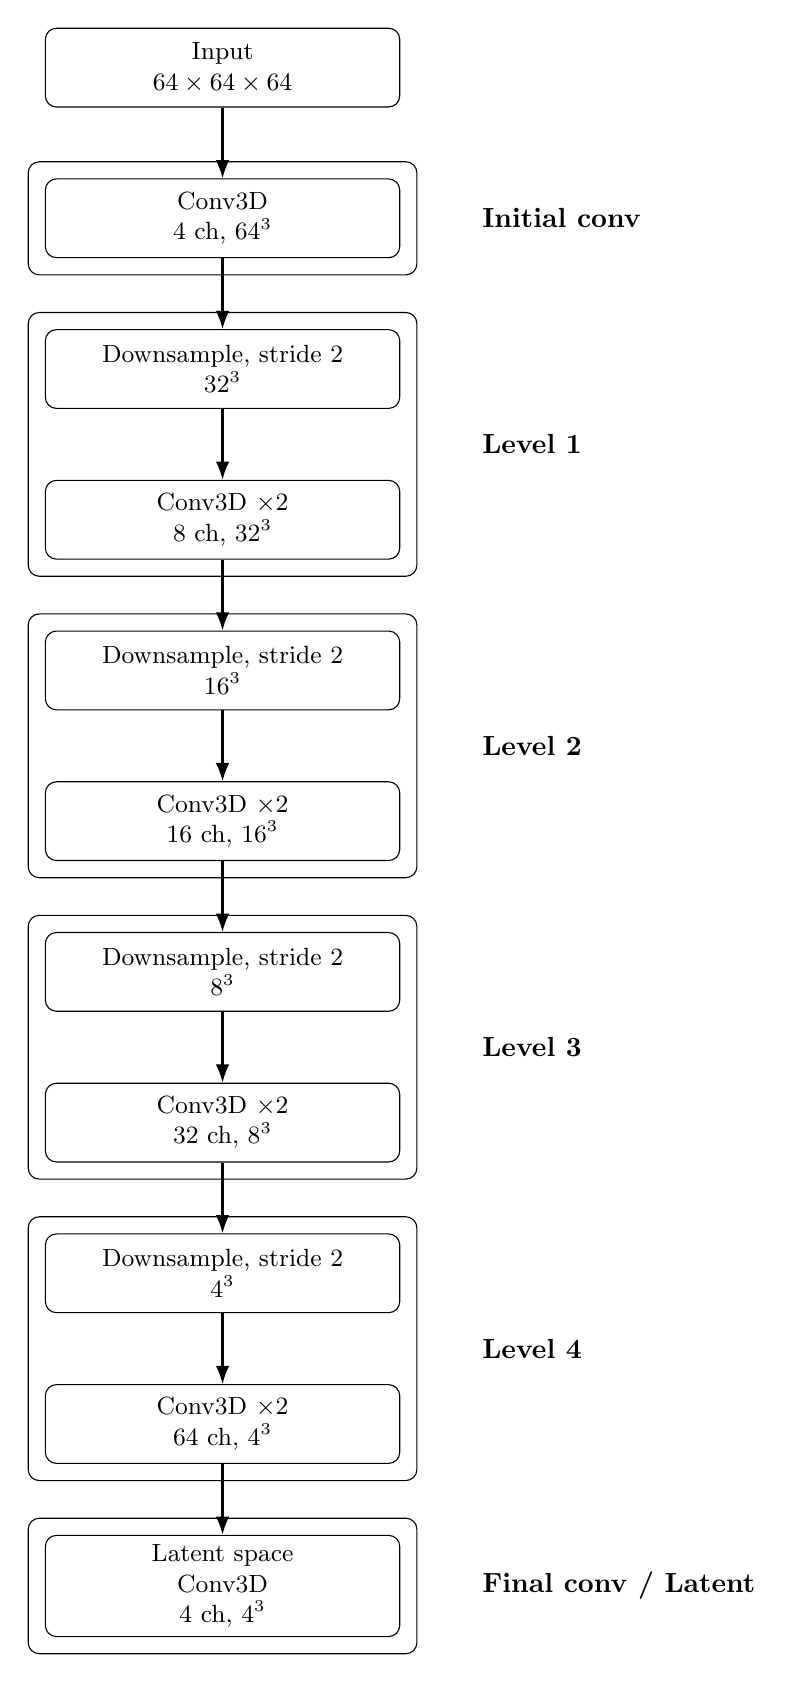
\begin{tikzpicture}[
    >=Latex,
    node distance = 0.9cm,
    block/.style   = {draw, rounded corners, minimum width=4.5cm,
                      minimum height=1.0cm, align=center, font=\small},
    levelbox/.style = {draw, rounded corners, inner sep=6pt},
    every edge/.style={draw,->,thick}
]

% =========================================================
% INPUT (KEEP THIS)
% =========================================================
\node[block] (input) {Input \\ $64 \times 64 \times 64$};

% =========================================================
% INITIAL CONV (KEEP THIS)
% =========================================================
\node[block, below=of input] (enc0) {Conv3D \\ 4 ch, $64^3$};
\node[levelbox, fit=(enc0)] (L0) {};
\node[right=0.7cm of L0] {\textbf{Initial conv}};

% =========================================================
% LEVEL 1  (YOU CAN DELETE / DUPLICATE THIS WHOLE BLOCK)
% =========================================================
\node[block, below=of enc0] (ds1)  {Downsample, stride 2 \\ $32^3$};
\node[block, below=of ds1]  (enc1) {Conv3D $\times 2$ \\ 8 ch, $32^3$};

\node[levelbox, fit=(ds1) (enc1)] (L1) {};
\node[right=0.7cm of L1] {\textbf{Level 1}};

% =========================================================
% LEVEL 2  (YOU CAN DELETE / DUPLICATE THIS WHOLE BLOCK)
% =========================================================
\node[block, below=of enc1] (ds2)  {Downsample, stride 2 \\ $16^3$};
\node[block, below=of ds2]  (enc2) {Conv3D $\times 2$ \\ 16 ch, $16^3$};

\node[levelbox, fit=(ds2) (enc2)] (L2) {};
\node[right=0.7cm of L2] {\textbf{Level 2}};

% =========================================================
% LEVEL 3  (YOU CAN DELETE / DUPLICATE THIS WHOLE BLOCK)
% =========================================================
\node[block, below=of enc2] (ds3)  {Downsample, stride 2 \\ $8^3$};
\node[block, below=of ds3]  (enc3) {Conv3D $\times 2$ \\ 32 ch, $8^3$};

\node[levelbox, fit=(ds3) (enc3)] (L3) {};
\node[right=0.7cm of L3] {\textbf{Level 3}};

% =========================================================
% LEVEL 4  (YOU CAN DELETE / DUPLICATE THIS WHOLE BLOCK)
% =========================================================
\node[block, below=of enc3] (ds4)  {Downsample, stride 2 \\ $4^3$};
\node[block, below=of ds4]  (enc4) {Conv3D $\times 2$ \\ 64 ch, $4^3$};

\node[levelbox, fit=(ds4) (enc4)] (L4) {};
\node[right=0.7cm of L4] {\textbf{Level 4}};

% =========================================================
% LATENT SPACE (KEEP THIS)
% =========================================================
\node[block, below=of enc4] (latent) {Latent space \\ Conv3D \\ 4 ch, $4^3$};
\node[levelbox, fit=(latent)] (L5) {};
\node[right=0.7cm of L5] {\textbf{Final conv / Latent}};

% =========================================================
% ARROWS
% =========================================================
\path
  (input)  edge (enc0)
  (enc0)   edge (ds1)
  (ds1)    edge (enc1)
  (enc1)   edge (ds2)
  (ds2)    edge (enc2)
  (enc2)   edge (ds3)
  (ds3)    edge (enc3)
  (enc3)   edge (ds4)
  (ds4)    edge (enc4)
  (enc4)   edge (latent);

\end{tikzpicture}
\end{center}

\end{document}
